\chapter{Ievads}
Ievadā ir jāietver:

\begin{itemize}
\item temata aktualitātes pamatojums;
\item darba mērķis;
\item darba mērķa sasniegšanai veicamo uzdevumu formulējums;
\item izmantojamo pētīšanas metožu un paņēmienu uzskaitījums;
\item literatūras un avotu grupu uzskaitījums (piemēram, speciālā ekonomiskā literatūra, valsts statistikas dati, nepublicētie materiāli no uzņēmuma arhīva u.c.);
\item darba struktūras apraksts;
\item pētījuma temata un perioda norobežojums (ja tas nepieciešams).
\end{itemize}

Mašīnmācīšanās algoritmi ir kļuvuši par neatņemamu sastāvdaļu programmatūras izstrādātājiem un kompānijām, kas savas aplikācijas grib padarīt "gudras". Lai arī cik, mūsdienās, šis jēdziens ir kļuvis populārs, oficiāla mašīnmācīšanās definīcija nav noteikta. Visvienkāršākais mašīnmācīšanās pielietojums ir apstrādāt datus, mācīties no tiem un no iegūtajiem rezultātiem pieņemt lēmumus vai veikt minējumus reālās pasaules problēmu risināšanai. Tā vietā, lai manuāli veidotu programmatūras risinājumus, kas veic kādu uzdevumu, tiek apmācīti datori vai citas ierīces, izmantojot lielus datu apjomus. 
\section{Mašīnmācīšanās pamatjēdziens}
Pasaulē ir daudz un dažādi mašīnmācīšanās algoritmi un katru dienu tiek publicēti simtiem jaunu algoritmu. Tos var sagrupēt pēc apmācības veida (vadītā apmācība (\textit{supervised learning}), nevadītā apmācība (\textit{unsupervised learning}), pusvadītā apmācība (\textit{semi-supervised learning})) kā arī pēc formas vai funkcijas līdzībām (klasifikācija, regresija, lēmumu koki (\textit{decision trees}), klasterēšana (\textit{clustering}), dziļā mašīnmācīšanās (\textit{deep learning})). Neatkarīgi no apmācības veida vai pielietojuma, visas mašīnmācīšanās algoritmu kombinācijas sastāv no klasifikatoriem (atbalsta vektora mašīna, lēmuma koki, neironu tīkli), vērtēšanas funkcijām (varbūtības funkcijas, robežfunkcijas, izmaksu funkcija) un optimizācijas funkcijām (mantkārīgā meklēšana, nepārtrauktās optimizācijas metodes (\textit{continuous optimization})). Izmantojot šīs sastāvdaļas, mašīnmācīšanās algoritmu pamata mērķis ir būt spējīgam funkcionēt ne tikai ar apmācībā piedāvātajiem datiem, bet arī spēt darboties ar datiem, ar kuriem algoritms nav saskāries. Atkarībā no veicamā uzdevuma, ir dažādi veidi kā panākt, lai datori vai jebkura cita ierīce mācās, sākot ar visparastākajiem lēmumu kokiem, beidzot ar ģenētiskajiem algoritmiem un mākslīgajiem neironu tīkliem. 


\newpage
\section{Datorredze}
Datorredze (no angļu val. \textit{computer vision}) ir datorzinātņu nozare, kuras mērķis ir ļaut datoriem redzēt un veikt tādus pašus uzdevumus kā cilvēki veiktu ar acīm un darīt to tikpat efektīvi. Redzes nodrošināšana datoriem nozīmē dot tiem spēju identificēt un apstrādāt attēlus līdzīgi kā to spēj darīt cilvēki. Tas ir kā nodot cilvēku inteliģenci un instinktus datoram. Datorredzes sistēmas parasti iedala trīs komponentēs:
\begin{itemize}
	\item Attēla iegūšana;
	\item Attēla apstrāde;
	\item Attēla analīze;
\end{itemize}
Līdzīgi kā cilvēku pasaules izpratne balstās uz spēju pieņemt lēmumus ņemot vērā redzēto, piedāvājot datoriem šādu vizuālu izpratni, tiem būtu iespējams pieņemt patstāvīgus lēmumus.

\begin{figure}[h]%
	\centering
	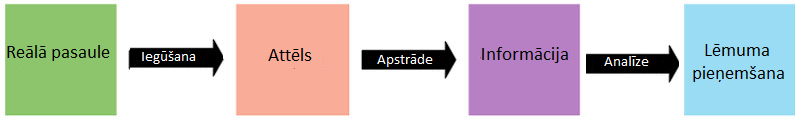
\includegraphics[height=2cm]{images/computervision1.png} %
	\caption{Datorredzes pamatprincips}%
	\label{fig:example}%
\end{figure}

Attēlu iegūšana ir process kurā reālās pasaules notikumi tiek pārveidoti bināros datos, kurus interpretē kā digitālus attēlus vai kā daļu no video fragmenta. 

Attēlu apstrāde ir iegūto attēlu zema līmeņa apstrāde. Pirmajā solī iegūtajiem binārajiem datiem pielieto algoritmus, kas norāda uz attēla daļām, kas satur zema līmeņa informāciju. Šādu informāciju var izšķirt pēc jebkādiem ģeometriskiem elementiem, kas sastāda attēlu, piemēram, punkti attēlā, attēla malas vai segmenti. Zema līmeņa attēlu apstrādes algoritmi ir malu detektēšana, segmentācijas algoritmi, klasifikācija, īpašību detektēšana.
\begin{figure}[h]%
	\centering
	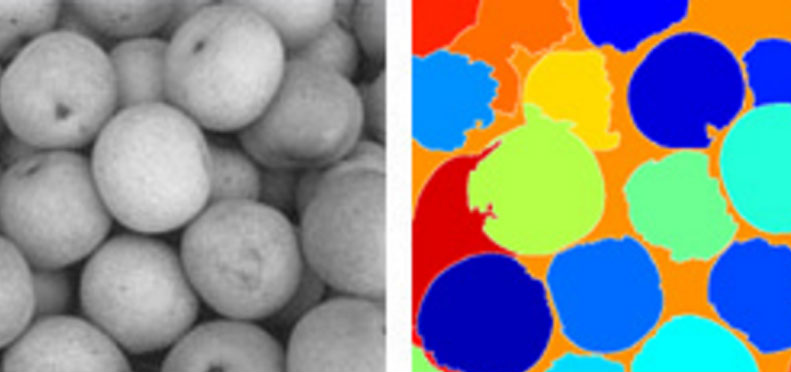
\includegraphics[height=3cm]{images/computervision2.png} %
	\caption{Ābolu segmentācija attēlā \cite{compv1}}%
	\label{fig:example}%
\end{figure} 

Pēdējā datorredzes sistēmu komponente ir attēlu analīzes solis, kurā notiks attēla analīze un pēc šī soļa datorredzes sistēmai būs iespējams pieņemt lēmumu un izvadē to atgriezt. Attēlu analīzes solī tiek pielietoti augsta līmeņa algoritmi, ņemot vērā gan attēla apstrādes solī iegūto zema līmeņa informāciju, gan pašu attēlu. Piemēri kur var izmantot šādu augsta līmeņa attēlu analīzi ir trīsdimensiju ainu atveidošana, objektu atpazīšana, objektu sekošana, cilvēku plūsmas analīze.
\begin{figure}[h]%
	\centering
	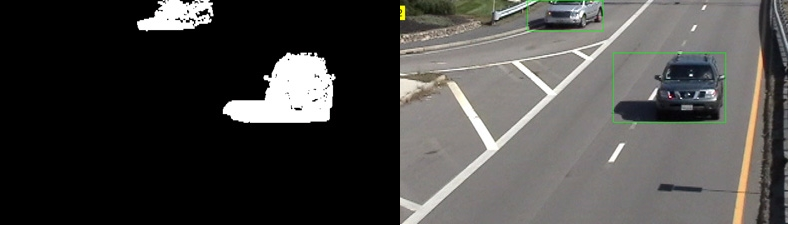
\includegraphics[height=4cm]{images/computervision3.png} %
	\caption{Objektu detektēšana pēc segmentācijas pielietošanas \cite{compv2}}%
	\label{fig:example}%
\end{figure} 

Izstrādājot datorredzes sistēmas, pētnieki saskaras ar dažādām problēmām un izaicinājumiem. Parasti šīs problēmas ir atkarīgas no datu kvalitātes, sistēmas pielietojuma un apkārtējās pasaules ietekmes uz datiem un aparatūru. Datorredzes pētnieki izstrādā risinājumus, lai padarītu datorredzes algoritmus stabilākus un efektīvākus sarežģītos uzstādījumos: nekvalitatīvi vai trokšņaini dati, reālā laika apstrāde un ierobežota skaitļošanas jauda. Mūsdienās, lai risinātu šīs problēmas, tiek savienoti mašīnmācīšanās risinājumi ar datorredzes risinājumiem.

Klasiskie datorredzes algoritmi ir smalki pētīti un optimizēti, lai iegūtu labāko veiktspēju un lai tie efektīvi izmantotu datora skaitļošanas resursus, kamēr mašīnmācīšanās algoritmi piedāvā precīzākus un vispusīgākus risinājumus, taču prasa lielus skaitļošanas resursus. Ņemot vērā iepriekš minēto, mūsdienu pētījumos ir populāri risinājumi, kas apvieno standarta datorredzes algoritmus un mašīnmācīšanās risinājumus. Labs piemērs abu šo nozaru apvienošanā ir kustīgu objektu meklēšana video fragmentos. Lai iegūtu augstāku precizitāti un taupītu skaitļošanas resursus ir iespējams attēla apstrādi veikt ar datorredzes algoritmiem un attēla analīzi (klasifikāciju, lokalizāciju, sekošanu) veikt ar neironu tīkliem.



